\documentclass[a4paper,12pt]{ctexart}
\usepackage{graphicx}
\usepackage{geometry}
\geometry{left=2.5cm, right=2.5cm, top=2.5cm, bottom=2.5cm}
\usepackage{titlesec}
\usepackage{float}
\usepackage{caption}

\title{\LARGE \textbf{实用新型专利申请说明书}}
\author{}
\date{}

\begin{document}

\maketitle

\section*{一、发明名称}
一种用于碳酸饮料快速物理去气的搅拌装置

\section*{二、技术领域}
本实用新型涉及生活餐饮用具及物理消泡技术领域，具体涉及一种无需添加化学试剂即可快速解析液体中溶解气体的便携式搅拌装置，尤其适用于碳酸饮料的快速物理去气。

\section*{三、背景技术}
在日常生活中，许多消费者（如胃部不适易胀气者、儿童、或需要利用碳酸饮料制作特定饮品/菜肴的人群）希望在饮用或使用碳酸饮料（如可乐、雪碧、苏打水等）时，能够快速去除其中的二氧化碳气体。

现有的去气方法通常包括：
1. 长时间静置，耗时极长；
2. 剧烈摇晃后开盖，极易导致液体喷溅和脏污；
3. 插入普通勺子或筷子进行搅拌，但普通餐具表面光滑，无法提供足够的成核位点，去气效率极低；
4. 添加表面活性剂（如糖果），但这会改变饮料原有的风味并可能引入化学添加剂。

因此，亟需一种便携、卫生、不改变饮品风味且能瞬间完成物理去气的装置。

\section*{四、权利要求书}
1. 一种用于含气饮料的物理去气搅拌装置，其特征在于，包括：
\begin{itemize}
    \item 手柄部（1），用于握持及搅拌操作；
    \item 工作部（2），设置于所述手柄部（1）的一端，用于浸入液体中；
    \item 连接部（3），用于将所述手柄部（1）与所述工作部（2）固定连接；
\end{itemize}
其中，所述工作部（2）由具有微观多孔结构的材料制成，所述手柄部（1）的表面粗糙度低于所述工作部（2）的表面粗糙度。

2. 根据权利要求1所述的物理去气搅拌装置，其特征在于，所述工作部（2）的微观多孔结构的孔径范围为 1 $\mu m$ 至 100 $\mu m$。

3. 根据权利要求2所述的物理去气搅拌装置，其特征在于，所述工作部（2）的微观多孔结构的孔径范围为 5 $\mu m$ 至 20 $\mu m$。

4. 根据权利要求1所述的物理去气搅拌装置，其特征在于，所述工作部（2）的材料选自粉末冶金烧结金属、多孔陶瓷或高分子微孔塑料中的一种。

5. 根据权利要求4所述的物理去气搅拌装置，其特征在于，所述工作部（2）的材料为 316L 不锈钢粉末烧结材料或 304 不锈钢粉末烧结材料。

6. 根据权利要求1所述的物理去气搅拌装置，其特征在于，所述手柄部（1）为金属杆、塑料杆或玻璃杆中的一种。

7. 根据权利要求1所述的物理去气搅拌装置，其特征在于，所述手柄部（1）为表面经过抛光处理的不锈钢实心杆。

8. 根据权利要求1所述的物理去气搅拌装置，其特征在于，所述连接部（3）采用焊接、螺纹连接、过盈配合或粘接中的一种方式将所述手柄部（1）与所述工作部（2）固定。

9. 根据权利要求1所述的物理去气搅拌装置，其特征在于，所述工作部（2）的外观呈圆柱形、水滴形或半球形。

10. 根据权利要求1所述的物理去气搅拌装置，其特征在于，所述工作部（2）的最大外径大于或等于所述手柄部（1）的外径。

\section*{五、实用新型内容}
本实用新型的目的在于克服现有技术的不足，提供一种用于碳酸饮料快速物理去气的搅拌装置。该装置利用特定的微观多孔物理结构，能够在浸入碳酸饮料时瞬间提供海量的气体成核位点，促使游离状态的二氧化碳迅速聚集成气泡并析出，实现快速、优雅的去气效果。

为实现上述目的，本实用新型采用如下技术方案：

一种用于碳酸饮料快速物理去气的搅拌装置，其特征在于，包括：
\begin{itemize}
    \item \textbf{手柄部（1）}：用于握持及搅拌操作，所述手柄部的表面为光滑无孔结构；
    \item \textbf{工作部（2）}：设置于所述手柄部的一端，用于浸入液体中，所述工作部由具有微观多孔结构的材料制成；
    \item \textbf{连接部（3）}：用于将所述手柄部与工作部固定连接。
\end{itemize}

作为本实用新型的进一步优化：
\begin{itemize}
    \item 所述工作部（2）的微观多孔结构的孔径范围为 $1\mu m$ 至 $100\mu m$。优选为 $5\mu m$ 至 $20\mu m$。
    \item 所述工作部（2）的材料选自粉末冶金烧结金属、多孔陶瓷或高分子微孔塑料中的一种。优选地，为316L医疗级或304食品级不锈钢粉末烧结材料。
    \item 所述手柄部（1）为实心或空心的金属杆、塑料杆或玻璃杆，其表面经过抛光或磨砂处理，其表面粗糙度低于所述工作部（2）。
    \item 所述连接部（3）采用焊接、螺纹连接、过盈配合或无毒食品级胶水粘接中的一种。
    \item 所述工作部（2）的外观呈圆柱形、水滴形或半球形，其最大外径与手柄部的外径相同或略大。
\end{itemize}

\section*{六、有益效果}
与现有技术相比，本实用新型具有以下有益效果：
1. \textbf{去气效率极高}：利用粉末烧结等多孔材料本身自带的千万级微孔，在液体中形成极其密集的“成核位点（Nucleation sites）”，插入碳酸饮料后数秒内即可使气体沸腾般溢出，去气速度远超普通搅拌棒。
2. \textbf{纯物理消泡，不改变风味}：无需添加任何化学消泡剂或糖分，100\% 保持饮品原本的味道与食品安全。
3. \textbf{视觉效果独特，防溢出}：光滑的手柄部不产生气泡，气泡仅集中在底部工作端产生，使用者可通过控制插入深度来精准控制放气速度，防止饮料剧烈喷溅。

\section*{七、附图说明}
\begin{figure}[H]
    \centering
    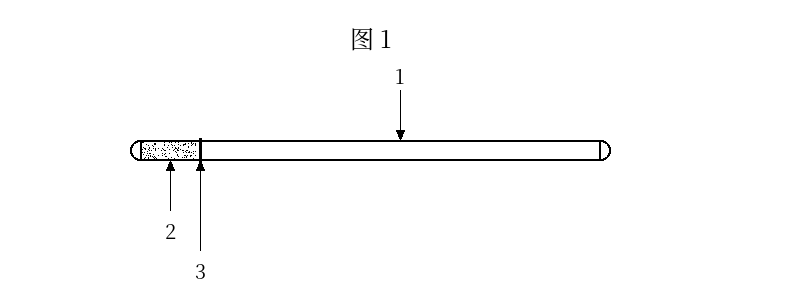
\includegraphics[width=0.8\textwidth]{FizzWand_Sketch.png}
    \caption{本实用新型搅拌装置的整体结构主视图草图。其中：1-手柄部；2-工作部（多孔烧结微孔端头）；3-连接部。}
\end{figure}

\begin{figure}[H]
    \centering
    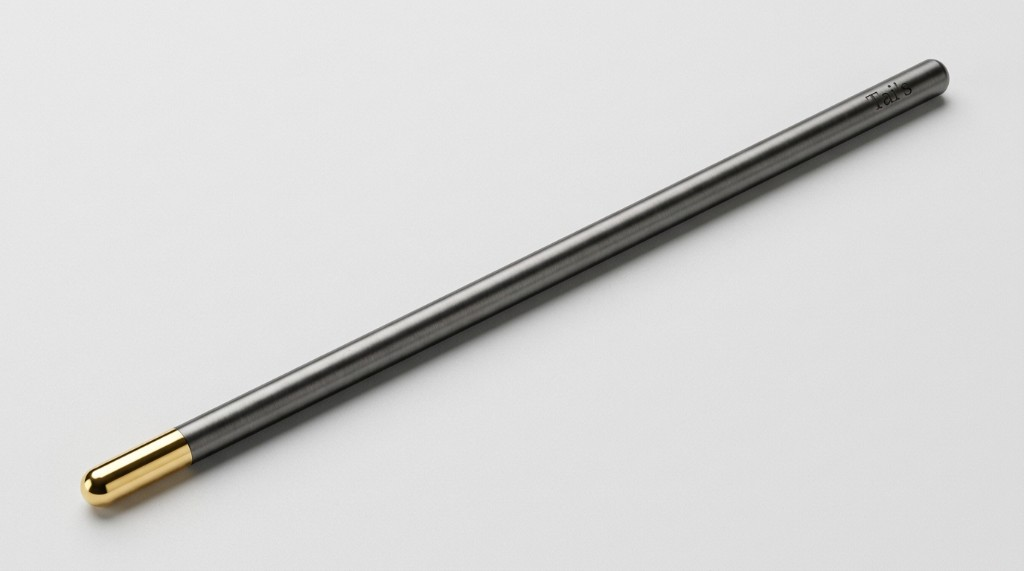
\includegraphics[width=0.8\textwidth]{FizzWand_Render.png}
    \caption{本实用新型搅拌装置的外观设计效果图（哑光杆身与金色多孔端头结合）。}
\end{figure}

\section*{八、具体实施方式}
为了使本实用新型的目的、技术方案及优点更加清楚明白，以下结合附图及实施例，对本实用新型进行进一步详细说明。

实施例1：
参照图1和图2，一种用于碳酸饮料快速去气的搅拌装置，总长度为 180mm。手柄部（1）为直径 6mm 的 304 不锈钢抛光实心圆棒，长度为 160mm。工作部（2）为直径 6mm、长度 20mm 的 316L 不锈钢烧结微孔端头，孔径为 10 微米，端部呈半球形倒角，外部采用镀钛工艺呈金色。连接部（3）采用激光无缝焊接工艺，将工作部（2）与手柄部（1）牢固连接，无卫生死角。

用户使用时，手持手柄部（1），将工作部（2）插入含有气体的碳酸饮料中。由于工作部（2）布满微孔，二氧化碳气体迅速在微孔处成核析出，轻微搅动 5-10 秒即可去除一杯 300ml 汽水中的绝大部分气体。此时手柄部（1）因表面光滑，不会引发大量气泡，从而保证握持处的整洁与气泡的可控性。

\end{document}